\documentclass[12pt,a4paper]{article}
\usepackage{fontspec}
\usepackage{xunicode}
\usepackage{xltxtra}
\usepackage{amsfonts}
\usepackage{comment}
\usepackage{graphicx}
\usepackage{float}
\usepackage{multirow}
\usepackage{lastpage}
\usepackage{fancyhdr}
\usepackage{hyperref}

\XeTeXlinebreaklocale “th”
\XeTeXlinebreakskip = 0pt plus 1pt
\defaultfontfeatures{Scale=1.4}
% !TeX spellcheck = en_US 
% !TeX spellcheck = TH 
\setmainfont{TH Sarabun New}
\title{Computational Science: SC313101 \\ Spring 2019}
\begin{document}
\maketitle 
\section{Instructor}
\begin{itemize}
	\item อ. ธนพล ตั้งชูพงศ์   Office (6325E)  Office Hours (xxxx)
	\item \href{ https://piazza.com/sc.kku.ac.th/spring2019/sc313101/} { Class website \\  piazza.com/sc.kku.ac.th/spring2019/sc313101/}
	
	\item \href{https://www.facebook.com/groups/225385098397971/}{ Facebook Group \\ www.facebook.com/groups/225385098397971 } 
	
	\item \href{https://github.com/thanaphon/ComputationalSC}{ Github for LAB documents: \\ https://github.com/thanaphon/ComputationalSC}
\end{itemize}
 





\section{Introduction}
	ยินดีตอนรับนักศึกษาทุกคนสู่คลาส Computational Science ในคลาสนี้ เนื้อหาจะครอบคลุมในส่วนของการใช้คอมพิวเตอร์เพื่อแก้ไขปัญหาทาง    วิทยาศาสตร์(Science), เทคโนโลยี (Technology), วิศวกรรม (Engineering), และ คณิตศาสตร์ (Mathematics)  โดยจะครอบคลุมถึงการทำ data analysis, visualization, simulation และ numerical analysis คลาสจะเริ่มโดย การรีวิวในส่วนของ Fundamental of programming โดยอาศัย Python  และใช้ ปัญหาทางวิทยาศาสตร์ มาเป็นโจทย์ในการเรียนรู้ ซึ่งจะโฟกัสในส่วนของแอฟฟลิแคชั่น เพื่อให้เห็นถึงการนำ ความรู้ที่ได้ไป บูรณาการ์ณกับปัญหาจริง        

\section{ Goals}
\begin{itemize}
	\item ช่วยสร้างความมันใจในการเขียนโปรแกรมให้นักศึกษา โดยการพัฒนาโปรแกรมขนาดเล็ก  
	\item แปลงปัญหาทางวิทยาศาตร์ ให้มาอยู่สูตรของการคำนวณสำหรับเฟรมเวอร์คที่เหมาะสม 
	\item เตรียมนักศึกษาได้รู้ถึงเทคนิคต่าง ๆ ที่ใช้ในวิธีทางการคำนวณ  เพื่อให้นักศึกษาสามารถนำไปประยุกใช้กับปัญหาเฉพาะที่นักศึกษาสนใจ 
	\item สามารถออกแบบและทำการทดลองโดยอาศัย computer simulation 
\end{itemize}

ซึ่งเราสามรถสรุป วัตถุประสงค์ข้างต้นเป็นหัวข้อที่นักศึกษาจะได้ เรียนรู้ดังต่อไปนี้
\begin{itemize}
	\item เรียนรู้การเขียนโปรแกรม เพื่อนำเสนอการคำนวณ โดยใช้ Python และ Matlab (Octave) รวมถึงการเรียกใช้ โมดูล Python ต่างๆ  
	\item เรียนรู้กระบวนการ ในการเขียนเเละดีบักโปรแกรม
	\item เรียนรู้กระบวนการในการแปลงปัญหาจาก โจทย์หรือ problem statement ไปยัง framework ที่ใช้แก้ไขปัญหา 
	\item เรียนในส่วนของอัลกอริทึม พื้นฐานที่ใช้ในงานสำหรับวิทยาการคำนวณ   
	\item เรียนรู้วิธีการในการใช้ computer simulation เพื่อหาคำตอบของปัญหาทางวิทยาศาสตร์
	\item เรียนรู้วิธีการสร้างแบบจำลอง (Modeling) และเข้าใจข้อมูลโดย อาศัยเครื่องมือทางการคำนวณ (computational tools) 

\end{itemize}

\section {References}
\begin{itemize}
	\item \href{https://hplgit.github.io/primer.html/doc/pub/half/book.pdf}{A Primer on Scientific
		Programming with Python}
	\begin{figure}[H]
		\centering
		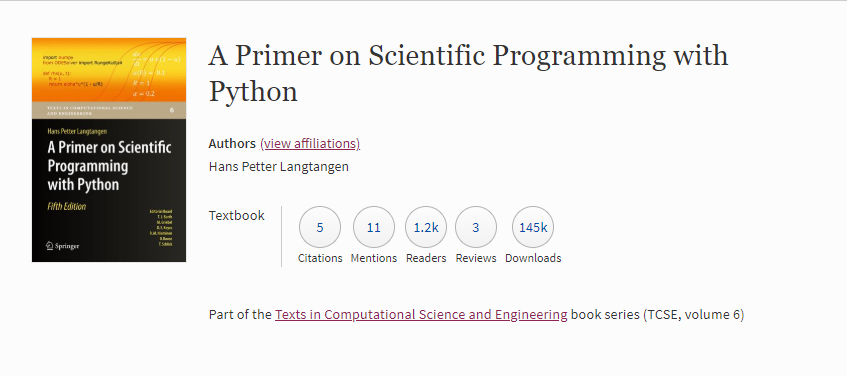
\includegraphics[width=0.7\linewidth]{PIC/book1}
		\caption{}
		\label{fig:book1}
	\end{figure}
	

\href{https://link.springer.com/book/10.1007/978-3-662-49887-3}{ลิงค์ไปยัง free download ของสำนักพิมพ์ ซึ่งนักศึกษาสามารถ part หลังของหนังสือได้ }
	
	
	\item \href{https://link.springer.com/book/10.1007%2F978-3-319-32428-9}{Free book อีกเล่มสำหรับ numerical excercises }
	\begin{figure} [H]
		\centering
		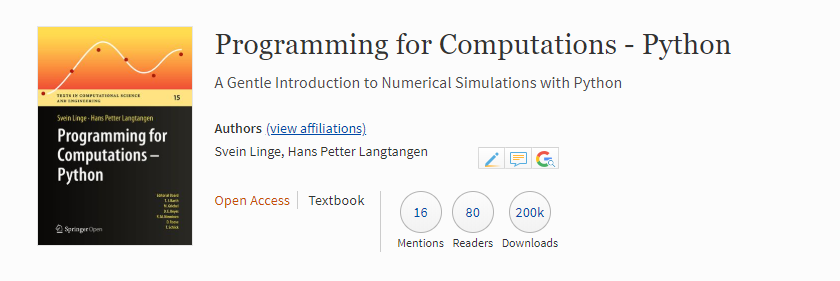
\includegraphics[width=0.7\linewidth]{PIC/book2}
		\caption{}
		\label{fig:book2}
	\end{figure}
	
\end{itemize}

\section{Grading schemes}
\begin{itemize}
	\item 40\%  Homework 
	\item 10\% Class participation
	\item 30\%  Exam
	\item 20\% Project 
\end{itemize}
\pagebreak
\section{Topics คร่าวๆ ซื่งอาจเปลี่ยนแปลงได้ ตามทิศทางความต้องการของนักศึกษา}
\begin{itemize}
	\item Motivation
	\subitem Type of scientific problems 
	\item Python programming
	\subitem lambda function, array manipulation, numpy, sympy (symbolic computing) 
	\subitem 
	เพื่อให้นักศึกษาคุ้นเคยกับ build in operators  และ modules ที่สำคัญ ๆ ของ Python ที่นิยมใช้ ในการแก้ปัญหาทางวิทยาศาสตร์ 
	\item Plotting graphs
	\subitem matplotlib, scitools
	\item Selected classical Numerical topics
	\begin{itemize}
		\item  Floating Point Arithmetic: Issues and Limitations \\ ( $0.1+0.1+0.1 == 0.3$ ) ? 
	
		\item Precision errors
		% https://docs.python.org/3/tutorial/floatingpoint.html
		\item Approximation functions: $sin x , cos x, e^x  $
		\item Controlling approximation error
		\item Root finding 
			\subitem ฺBisection search
		\subitem Newton method 
	\end{itemize}
	\item Probability and Information Theory
	\subitem เพื่อให้นักศึกษาคุ้นเคยกับ Histogram และ สามารถ เปลี่ยน raw data ให้อยู่ในรูปแบบของ distributions  สามารถนำข้อมูลที่กำหนดให้มาคำนวณหา information theory ของข้อมูล หรือหาความสัมพันธ์ ของข้องมูลอย่างง่าย
	\item Stochastic Methods
	\subitem Random number
	\subitem Monte Carlo method
	\subitem Markov Chain
	\subitem เพื่อให้นักศึกษามีพื้นฐานในการสร้างแบบจำลองเพื่อสร้าง  ฐานข้อมูล  โดยอาศัยโมเดลแบบ non-deterministic 
	\item System of linear equations 
	\subitem Matrix and Vector
	\subitem Numerical method for linear system equation
	\subitem Least square method
	\subitem  ให้นักศึกษาคุ้นเคยกับการเขียน โปรแกรมเพื่อจัดการกับขอมูขที่เป็น Matrix และ Vectors ต่าง สามารถนำข้อมูลจาก section ก่อนหน้ามาวิเคราะห์ เพื่อทำเเบบจำลอง ในรูปของ linear model 
	\item Computational Graph (optional)
	\item Modeling (optional)
	\subitem Epidemic models
	% https://leif.me/2016/12/on-the-diffusion-of-innovations-how-new-ideas-spread/
	
	\subitem Wave Equation
	  %https://www.maa.org/press/periodicals/loci/joma/the-sir-model-for-spread-of-disease-the-differential-equation-model
	  
\end{itemize}


\end{document}
